% Options for packages loaded elsewhere
\PassOptionsToPackage{unicode}{hyperref}
\PassOptionsToPackage{hyphens}{url}
%
\documentclass[
]{article}
\title{June\_2}
\author{Hainan Xu}
\date{02/06/2022}

\usepackage{amsmath,amssymb}
\usepackage{lmodern}
\usepackage{iftex}
\ifPDFTeX
  \usepackage[T1]{fontenc}
  \usepackage[utf8]{inputenc}
  \usepackage{textcomp} % provide euro and other symbols
\else % if luatex or xetex
  \usepackage{unicode-math}
  \defaultfontfeatures{Scale=MatchLowercase}
  \defaultfontfeatures[\rmfamily]{Ligatures=TeX,Scale=1}
\fi
% Use upquote if available, for straight quotes in verbatim environments
\IfFileExists{upquote.sty}{\usepackage{upquote}}{}
\IfFileExists{microtype.sty}{% use microtype if available
  \usepackage[]{microtype}
  \UseMicrotypeSet[protrusion]{basicmath} % disable protrusion for tt fonts
}{}
\makeatletter
\@ifundefined{KOMAClassName}{% if non-KOMA class
  \IfFileExists{parskip.sty}{%
    \usepackage{parskip}
  }{% else
    \setlength{\parindent}{0pt}
    \setlength{\parskip}{6pt plus 2pt minus 1pt}}
}{% if KOMA class
  \KOMAoptions{parskip=half}}
\makeatother
\usepackage{xcolor}
\IfFileExists{xurl.sty}{\usepackage{xurl}}{} % add URL line breaks if available
\IfFileExists{bookmark.sty}{\usepackage{bookmark}}{\usepackage{hyperref}}
\hypersetup{
  pdftitle={June\_2},
  pdfauthor={Hainan Xu},
  hidelinks,
  pdfcreator={LaTeX via pandoc}}
\urlstyle{same} % disable monospaced font for URLs
\usepackage[margin=1in]{geometry}
\usepackage{color}
\usepackage{fancyvrb}
\newcommand{\VerbBar}{|}
\newcommand{\VERB}{\Verb[commandchars=\\\{\}]}
\DefineVerbatimEnvironment{Highlighting}{Verbatim}{commandchars=\\\{\}}
% Add ',fontsize=\small' for more characters per line
\usepackage{framed}
\definecolor{shadecolor}{RGB}{248,248,248}
\newenvironment{Shaded}{\begin{snugshade}}{\end{snugshade}}
\newcommand{\AlertTok}[1]{\textcolor[rgb]{0.94,0.16,0.16}{#1}}
\newcommand{\AnnotationTok}[1]{\textcolor[rgb]{0.56,0.35,0.01}{\textbf{\textit{#1}}}}
\newcommand{\AttributeTok}[1]{\textcolor[rgb]{0.77,0.63,0.00}{#1}}
\newcommand{\BaseNTok}[1]{\textcolor[rgb]{0.00,0.00,0.81}{#1}}
\newcommand{\BuiltInTok}[1]{#1}
\newcommand{\CharTok}[1]{\textcolor[rgb]{0.31,0.60,0.02}{#1}}
\newcommand{\CommentTok}[1]{\textcolor[rgb]{0.56,0.35,0.01}{\textit{#1}}}
\newcommand{\CommentVarTok}[1]{\textcolor[rgb]{0.56,0.35,0.01}{\textbf{\textit{#1}}}}
\newcommand{\ConstantTok}[1]{\textcolor[rgb]{0.00,0.00,0.00}{#1}}
\newcommand{\ControlFlowTok}[1]{\textcolor[rgb]{0.13,0.29,0.53}{\textbf{#1}}}
\newcommand{\DataTypeTok}[1]{\textcolor[rgb]{0.13,0.29,0.53}{#1}}
\newcommand{\DecValTok}[1]{\textcolor[rgb]{0.00,0.00,0.81}{#1}}
\newcommand{\DocumentationTok}[1]{\textcolor[rgb]{0.56,0.35,0.01}{\textbf{\textit{#1}}}}
\newcommand{\ErrorTok}[1]{\textcolor[rgb]{0.64,0.00,0.00}{\textbf{#1}}}
\newcommand{\ExtensionTok}[1]{#1}
\newcommand{\FloatTok}[1]{\textcolor[rgb]{0.00,0.00,0.81}{#1}}
\newcommand{\FunctionTok}[1]{\textcolor[rgb]{0.00,0.00,0.00}{#1}}
\newcommand{\ImportTok}[1]{#1}
\newcommand{\InformationTok}[1]{\textcolor[rgb]{0.56,0.35,0.01}{\textbf{\textit{#1}}}}
\newcommand{\KeywordTok}[1]{\textcolor[rgb]{0.13,0.29,0.53}{\textbf{#1}}}
\newcommand{\NormalTok}[1]{#1}
\newcommand{\OperatorTok}[1]{\textcolor[rgb]{0.81,0.36,0.00}{\textbf{#1}}}
\newcommand{\OtherTok}[1]{\textcolor[rgb]{0.56,0.35,0.01}{#1}}
\newcommand{\PreprocessorTok}[1]{\textcolor[rgb]{0.56,0.35,0.01}{\textit{#1}}}
\newcommand{\RegionMarkerTok}[1]{#1}
\newcommand{\SpecialCharTok}[1]{\textcolor[rgb]{0.00,0.00,0.00}{#1}}
\newcommand{\SpecialStringTok}[1]{\textcolor[rgb]{0.31,0.60,0.02}{#1}}
\newcommand{\StringTok}[1]{\textcolor[rgb]{0.31,0.60,0.02}{#1}}
\newcommand{\VariableTok}[1]{\textcolor[rgb]{0.00,0.00,0.00}{#1}}
\newcommand{\VerbatimStringTok}[1]{\textcolor[rgb]{0.31,0.60,0.02}{#1}}
\newcommand{\WarningTok}[1]{\textcolor[rgb]{0.56,0.35,0.01}{\textbf{\textit{#1}}}}
\usepackage{graphicx}
\makeatletter
\def\maxwidth{\ifdim\Gin@nat@width>\linewidth\linewidth\else\Gin@nat@width\fi}
\def\maxheight{\ifdim\Gin@nat@height>\textheight\textheight\else\Gin@nat@height\fi}
\makeatother
% Scale images if necessary, so that they will not overflow the page
% margins by default, and it is still possible to overwrite the defaults
% using explicit options in \includegraphics[width, height, ...]{}
\setkeys{Gin}{width=\maxwidth,height=\maxheight,keepaspectratio}
% Set default figure placement to htbp
\makeatletter
\def\fps@figure{htbp}
\makeatother
\setlength{\emergencystretch}{3em} % prevent overfull lines
\providecommand{\tightlist}{%
  \setlength{\itemsep}{0pt}\setlength{\parskip}{0pt}}
\setcounter{secnumdepth}{-\maxdimen} % remove section numbering
\ifLuaTeX
  \usepackage{selnolig}  % disable illegal ligatures
\fi

\begin{document}
\maketitle

\hypertarget{preliminary-tresholding-for-mbp-june2}{%
\subsection{Preliminary Tresholding for MBP
(June2)}\label{preliminary-tresholding-for-mbp-june2}}

Load the package and read the image.

\begin{Shaded}
\begin{Highlighting}[]
\FunctionTok{library}\NormalTok{(BiocManager)}
\end{Highlighting}
\end{Shaded}

\begin{verbatim}
## Bioconductor version '3.14' is out-of-date; the current release version '3.15'
##   is available with R version '4.2'; see https://bioconductor.org/install
\end{verbatim}

\begin{Shaded}
\begin{Highlighting}[]
\FunctionTok{library}\NormalTok{(EBImage)}
\NormalTok{im}\OtherTok{=}\FunctionTok{readImage}\NormalTok{(}\StringTok{"/Users/hainanxu/Documents/spatial\_visual\_cortex/data/im3.jpg"}\NormalTok{)}
\end{Highlighting}
\end{Shaded}

Check the histogram, we can see that there are 3 colors in the
histogram, and they are interlaced. Therefore, we need to convert the
color mode to greyscale.
\includegraphics{Thresholding-MBP_June3_files/figure-latex/pressure-1.pdf}
Take a look at \texttt{r}。

\begin{Shaded}
\begin{Highlighting}[]
\FunctionTok{display}\NormalTok{(r)}
\end{Highlighting}
\end{Shaded}

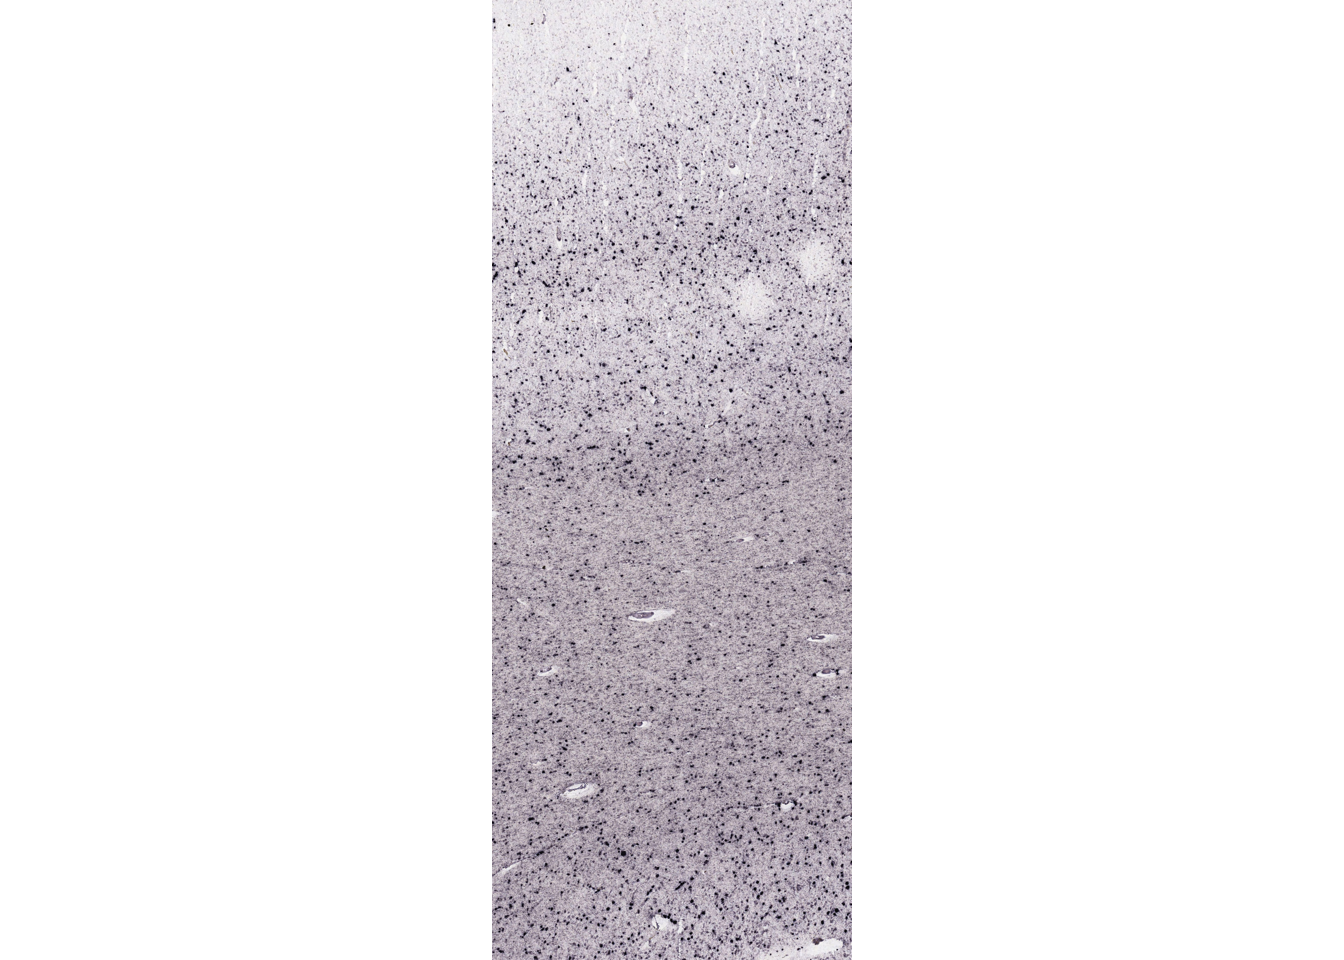
\includegraphics{Thresholding-MBP_June3_files/figure-latex/unnamed-chunk-1-1.pdf}

\begin{Shaded}
\begin{Highlighting}[]
\CommentTok{\#w = makeBrush(size = 30, shape = "gaussian", sigma = 2)}
\CommentTok{\#nucSmooth = filter2(getFrame(r, 1), w)}
\CommentTok{\#display(nucSmooth)}
\CommentTok{\#display(nucSmooth\textless{}0.3)}
\end{Highlighting}
\end{Shaded}

Threshold the \texttt{r} and do open operation.

\begin{Shaded}
\begin{Highlighting}[]
\FunctionTok{hist}\NormalTok{(r)}
\end{Highlighting}
\end{Shaded}

\includegraphics{Thresholding-MBP_June3_files/figure-latex/unnamed-chunk-2-1.pdf}

\begin{Shaded}
\begin{Highlighting}[]
\FunctionTok{display}\NormalTok{(r}\SpecialCharTok{\textless{}}\FloatTok{0.3}\NormalTok{)}
\end{Highlighting}
\end{Shaded}

\includegraphics{Thresholding-MBP_June3_files/figure-latex/unnamed-chunk-2-2.pdf}

\begin{Shaded}
\begin{Highlighting}[]
\NormalTok{rThresh}\OtherTok{=}\NormalTok{r}\SpecialCharTok{\textless{}}\FloatTok{0.3}
\NormalTok{rOpened }\OtherTok{=}\NormalTok{ EBImage}\SpecialCharTok{::}\FunctionTok{opening}\NormalTok{(rThresh,}
                            \AttributeTok{kern =} \FunctionTok{makeBrush}\NormalTok{(}\DecValTok{3}\NormalTok{, }\AttributeTok{shape =} \StringTok{"disc"}\NormalTok{))}
\FunctionTok{display}\NormalTok{(rOpened)}
\end{Highlighting}
\end{Shaded}

\includegraphics{Thresholding-MBP_June3_files/figure-latex/unnamed-chunk-2-3.pdf}

\begin{Shaded}
\begin{Highlighting}[]
\NormalTok{rRGB}\OtherTok{=}\FunctionTok{toRGB}\NormalTok{(rOpened)}
\FunctionTok{writeImage}\NormalTok{(rRGB, }\StringTok{"Ahad\_June3.tiff"}\NormalTok{, }\AttributeTok{quality =} \DecValTok{100}\NormalTok{)}
\end{Highlighting}
\end{Shaded}

\begin{Shaded}
\begin{Highlighting}[]
\NormalTok{rSeed }\OtherTok{=} \FunctionTok{bwlabel}\NormalTok{(rOpened)}
\FunctionTok{display}\NormalTok{(}\FunctionTok{colorLabels}\NormalTok{(rSeed))}
\end{Highlighting}
\end{Shaded}

\includegraphics{Thresholding-MBP_June3_files/figure-latex/unnamed-chunk-3-1.pdf}

\begin{Shaded}
\begin{Highlighting}[]
\FunctionTok{table}\NormalTok{(rSeed)}
\end{Highlighting}
\end{Shaded}

\begin{verbatim}
## rSeed
##      0      1      2      3      4      5      6      7      8      9     10 
## 414719      6      9     65    106     48    117    191     47     98    119 
##     11     12     13     14     15     16     17     18     19     20     21 
##     29      9    109    103     63     57    105     95     66     27     62 
##     22     23     24     25     26     27     28     29     30     31     32 
##    103    112     92      9    116    157     50     62     63    194     89 
##     33     34     35     36     37     38     39     40     41     42     43 
##     38    110     68     39    150     53     39     12     46     66      9 
##     44     45     46     47     48     49     50     51     52     53     54 
##     61     92     57     57    172     27     28     22    212     28    186 
##     55     56     57     58     59     60     61     62     63     64     65 
##     65     15     44    154     15    224     82     47     43     81    101 
##     66     67     68     69     70     71     72     73     74     75     76 
##     61     22     30    221    179    109     97     56     46     72     87 
##     77     78     79     80     81     82     83     84     85     86     87 
##    167     71     91     55      6     56    116     55     88    110     46 
##     88     89     90     91     92     93     94     95     96     97     98 
##     15     55    189     55      9     25     67     71     18    196      9 
##     99    100    101    102    103    104    105    106    107    108    109 
##    114     25    143     16     16     19     27     28     79     75     61 
##    110    111    112    113    114    115    116    117    118    119    120 
##    111    133    206     19    107     56     90     65     15     64     12 
##    121    122    123    124    125    126    127    128    129    130    131 
##     34     12     12     15     82    113      9     85     79     85     95 
##    132    133    134    135    136    137    138    139    140    141    142 
##     19     72     71     18     62     18     97    117      9     45     15
\end{verbatim}

Threshold G and compare it with R.

\begin{Shaded}
\begin{Highlighting}[]
\FunctionTok{hist}\NormalTok{(r)}
\end{Highlighting}
\end{Shaded}

\includegraphics{Thresholding-MBP_June3_files/figure-latex/unnamed-chunk-4-1.pdf}

\begin{Shaded}
\begin{Highlighting}[]
\FunctionTok{display}\NormalTok{(g}\SpecialCharTok{\textless{}}\FloatTok{0.3}\NormalTok{)}
\end{Highlighting}
\end{Shaded}

\includegraphics{Thresholding-MBP_June3_files/figure-latex/unnamed-chunk-4-2.pdf}

\begin{Shaded}
\begin{Highlighting}[]
\NormalTok{rThresh}\OtherTok{=}\NormalTok{r}\SpecialCharTok{\textless{}}\FloatTok{0.3}
\NormalTok{rOpened }\OtherTok{=}\NormalTok{ EBImage}\SpecialCharTok{::}\FunctionTok{opening}\NormalTok{(rThresh,}
                            \AttributeTok{kern =} \FunctionTok{makeBrush}\NormalTok{(}\DecValTok{3}\NormalTok{, }\AttributeTok{shape =} \StringTok{"disc"}\NormalTok{))}
\FunctionTok{display}\NormalTok{(rOpened)}
\end{Highlighting}
\end{Shaded}

\includegraphics{Thresholding-MBP_June3_files/figure-latex/unnamed-chunk-4-3.pdf}

\begin{Shaded}
\begin{Highlighting}[]
\FunctionTok{writeImage}\NormalTok{(rOpened, }\StringTok{"Ahad\_June2.jpeg"}\NormalTok{, }\AttributeTok{quality =} \DecValTok{100}\NormalTok{)}
\end{Highlighting}
\end{Shaded}


\end{document}
